\documentclass[11pt]{article}
\usepackage{fullpage,amsthm,amsfonts,amssymb,epsfig,amsmath,times,amsthm,array,graphicx}
\newcolumntype{C}{>$c<$}
\usepackage[shortlabels]{enumitem}
\usepackage{mathtools}
\graphicspath{ {images/} }
\DeclarePairedDelimiter\ceil{\lceil}{\rceil}
\DeclarePairedDelimiter\floor{\lfloor}{\rfloor}

\newtheorem{theorem}{Theorem}
\newtheorem{claim}[theorem]{Claim}
\newtheorem*{claim*}{Claim}

\begin{document}

\begin{center}
{\bf\Large CMPS 130 -- Spring Quarter 2017 --  Homework 1}\\
Christopher Hsiao -- chhsiao@ucsc.edu -- 1398305\\
\end{center}



\section{Exercises from pages 25, 26, and 27 of the book: 0.1 through 0.9}
\subsection*{0.1} 
Examine the following formal descriptions of sets so that you understand which members they contain. Write a short informal English description of each set.

\begin{enumerate}[a.]
\item The infinite set of all positive odd integers, or the set of all odd natural numbers.
\item The infinite set of all even integers.
\item The infinite set of all even natural numbers.
\item The infinite set of all even natural numbers, and all natural numbers which are multiples of 3.
\item The infinite set containing all palindromic bit strings.
\item The finite set containing any integer $n$ and $n+1$. ========
\end{enumerate}

\subsection*{0.2}
Write formal descriptions of the following sets.

\begin{enumerate}[a.]
\item $\{1, 10, 100\}$
\item $\{n | n > 5 \text{ for some } n \in \mathbb{Z}\}$
\item $\{1, 2, 3, 4\}$
\item $\{aba\}$
\item $\{""\}$
\item $\{ \}$
\end{enumerate}

\subsection*{0.3}
Let $A$ be the set $\{x, y, z\}$ and $B$ be the set $\{x, y\}$.

\begin{enumerate}[a.]
\item No.
\item Yes.
\item $\{x, y, z\}$
\item $\{x, y\}$
\item \{\{x,x\}, \{x,y\}, \{y,x\}, \{y, y\}, \{z, x\}, \{z, y\}\}
\item \{\{\}, \{x\}, \{y\}, \{x,y\}\}
\end{enumerate}

\subsection*{0.4}
If $A$ has $a$ elements, and $B$ has $b$ elements, how many elements are in $A \times B$? Explain your answer.\\
\begin{claim*}
$|A \times B| = a \cdot b$ 
\end{claim*}
\begin{proof}
This is because we assign every element of the set $A$ to every element in the set $B$. That means, each element in the set $A$, such as $A_i$, has $b$ pairings made. Thus, if there are $b$ pairings made with every element in $A$, then there are $a$ pairings, each of size $b$, which yields $a \cdot b$ number of pairings made. 
\end{proof}

\subsection*{0.5}
If $C$ is a set with $c$ elements, how many elements are in the power set of $C$? Explain your answer.\\
\\
First, we will define the power set of $C$ as $P_C$. 
\begin{claim*}
$|P_C| = 2^{c}$
\end{claim*}
\begin{proof}

\end{proof}

\subsection*{0.6}
Let X be the set $\{1, 2, 3, 4, 5\}$ and $Y$ be the set $\{6, 7, 8, 9, 10\}$. The unary function $f: X \rightarrow Y$ and the binary function $g: X \times Y \rightarrow Y$ are described.

\begin{enumerate}[a.]
\item 7
\item $D: [6,7]$, $R: [1,5]$
\item 6
\item $D: [6,10]$, $R: [1,5]$
\item 8
\end{enumerate}

\subsection*{0.7}
For each part, give a relation that satisfies the condition. Let A = \{x, y, z\}.
\begin{enumerate}[a.]
\item Reflexive, Symmetric, but not Transitive. \\
Let $R$ = \{(x, x), (y, y), (z, z), (x, y), (y, x), (y, z), (z, y)\}\\
$R$ is reflexive, since (x, x), (y, y), (z, z) $\in R$.\\
$R$ is symmetric, since (x, y), (y, x), (y, z), (z, y) $\in R$.\\
$R$ is not transitive, since (x, y) (y, z) $\in R$, but (x, z) $\notin R$.
\item Reflexive, Transitive, but not Symmetric. \\
Let $R$ = \{(x, x), (y, y), (z, z), (x, y), (y, z), (x, z)\}\\
$R$ is reflexive, since (x, x), (y, y), (z, z) $\in R$.\\
$R$ is transitive, since (x, y), (y, z), (x, z) $\in R$, where (x, y) and (y, z) $\implies$ (x, z)\\
$R$ is not symmetric, since (x, y), (y, z), (x, z) $\in R$, but (y, x), (z, y), (z, x) $\notin R$.
\item Symmetric, Transitive, but not Reflexive.\\
Let $R$ = \{(x, y), (y, x), (y, z), (z, y), (x, z), (z, x)\}\\
$R$ is symmetric, since (x, y), (y, x), (y, z), (x, z), (z, x) $\in R$.\\
$R$ is transitive, since (x, y), (y, z), (z, x) $\in R$, where (x, y) and (y, z) $\implies$ (z, x).\\
$R$ is not reflexive, since (x, x), (y, y), (z, z) $\notin R$.
\end{enumerate}

\subsection*{0.8}
Consider the undirected graph $G=(V,E) where V$ , the set of nodes, is \{1, 2, 3, 4\} and $E$, the set of edges, is \{\{1, 2\}, \{2, 3\}, \{1, 3\}, \{2, 4\}, \{1, 4\}\}. Draw the graph $G$. What are the degrees of each node? Indicate a path from node 3 to
node 4 on your drawing of $G$.\\
\begin{center} 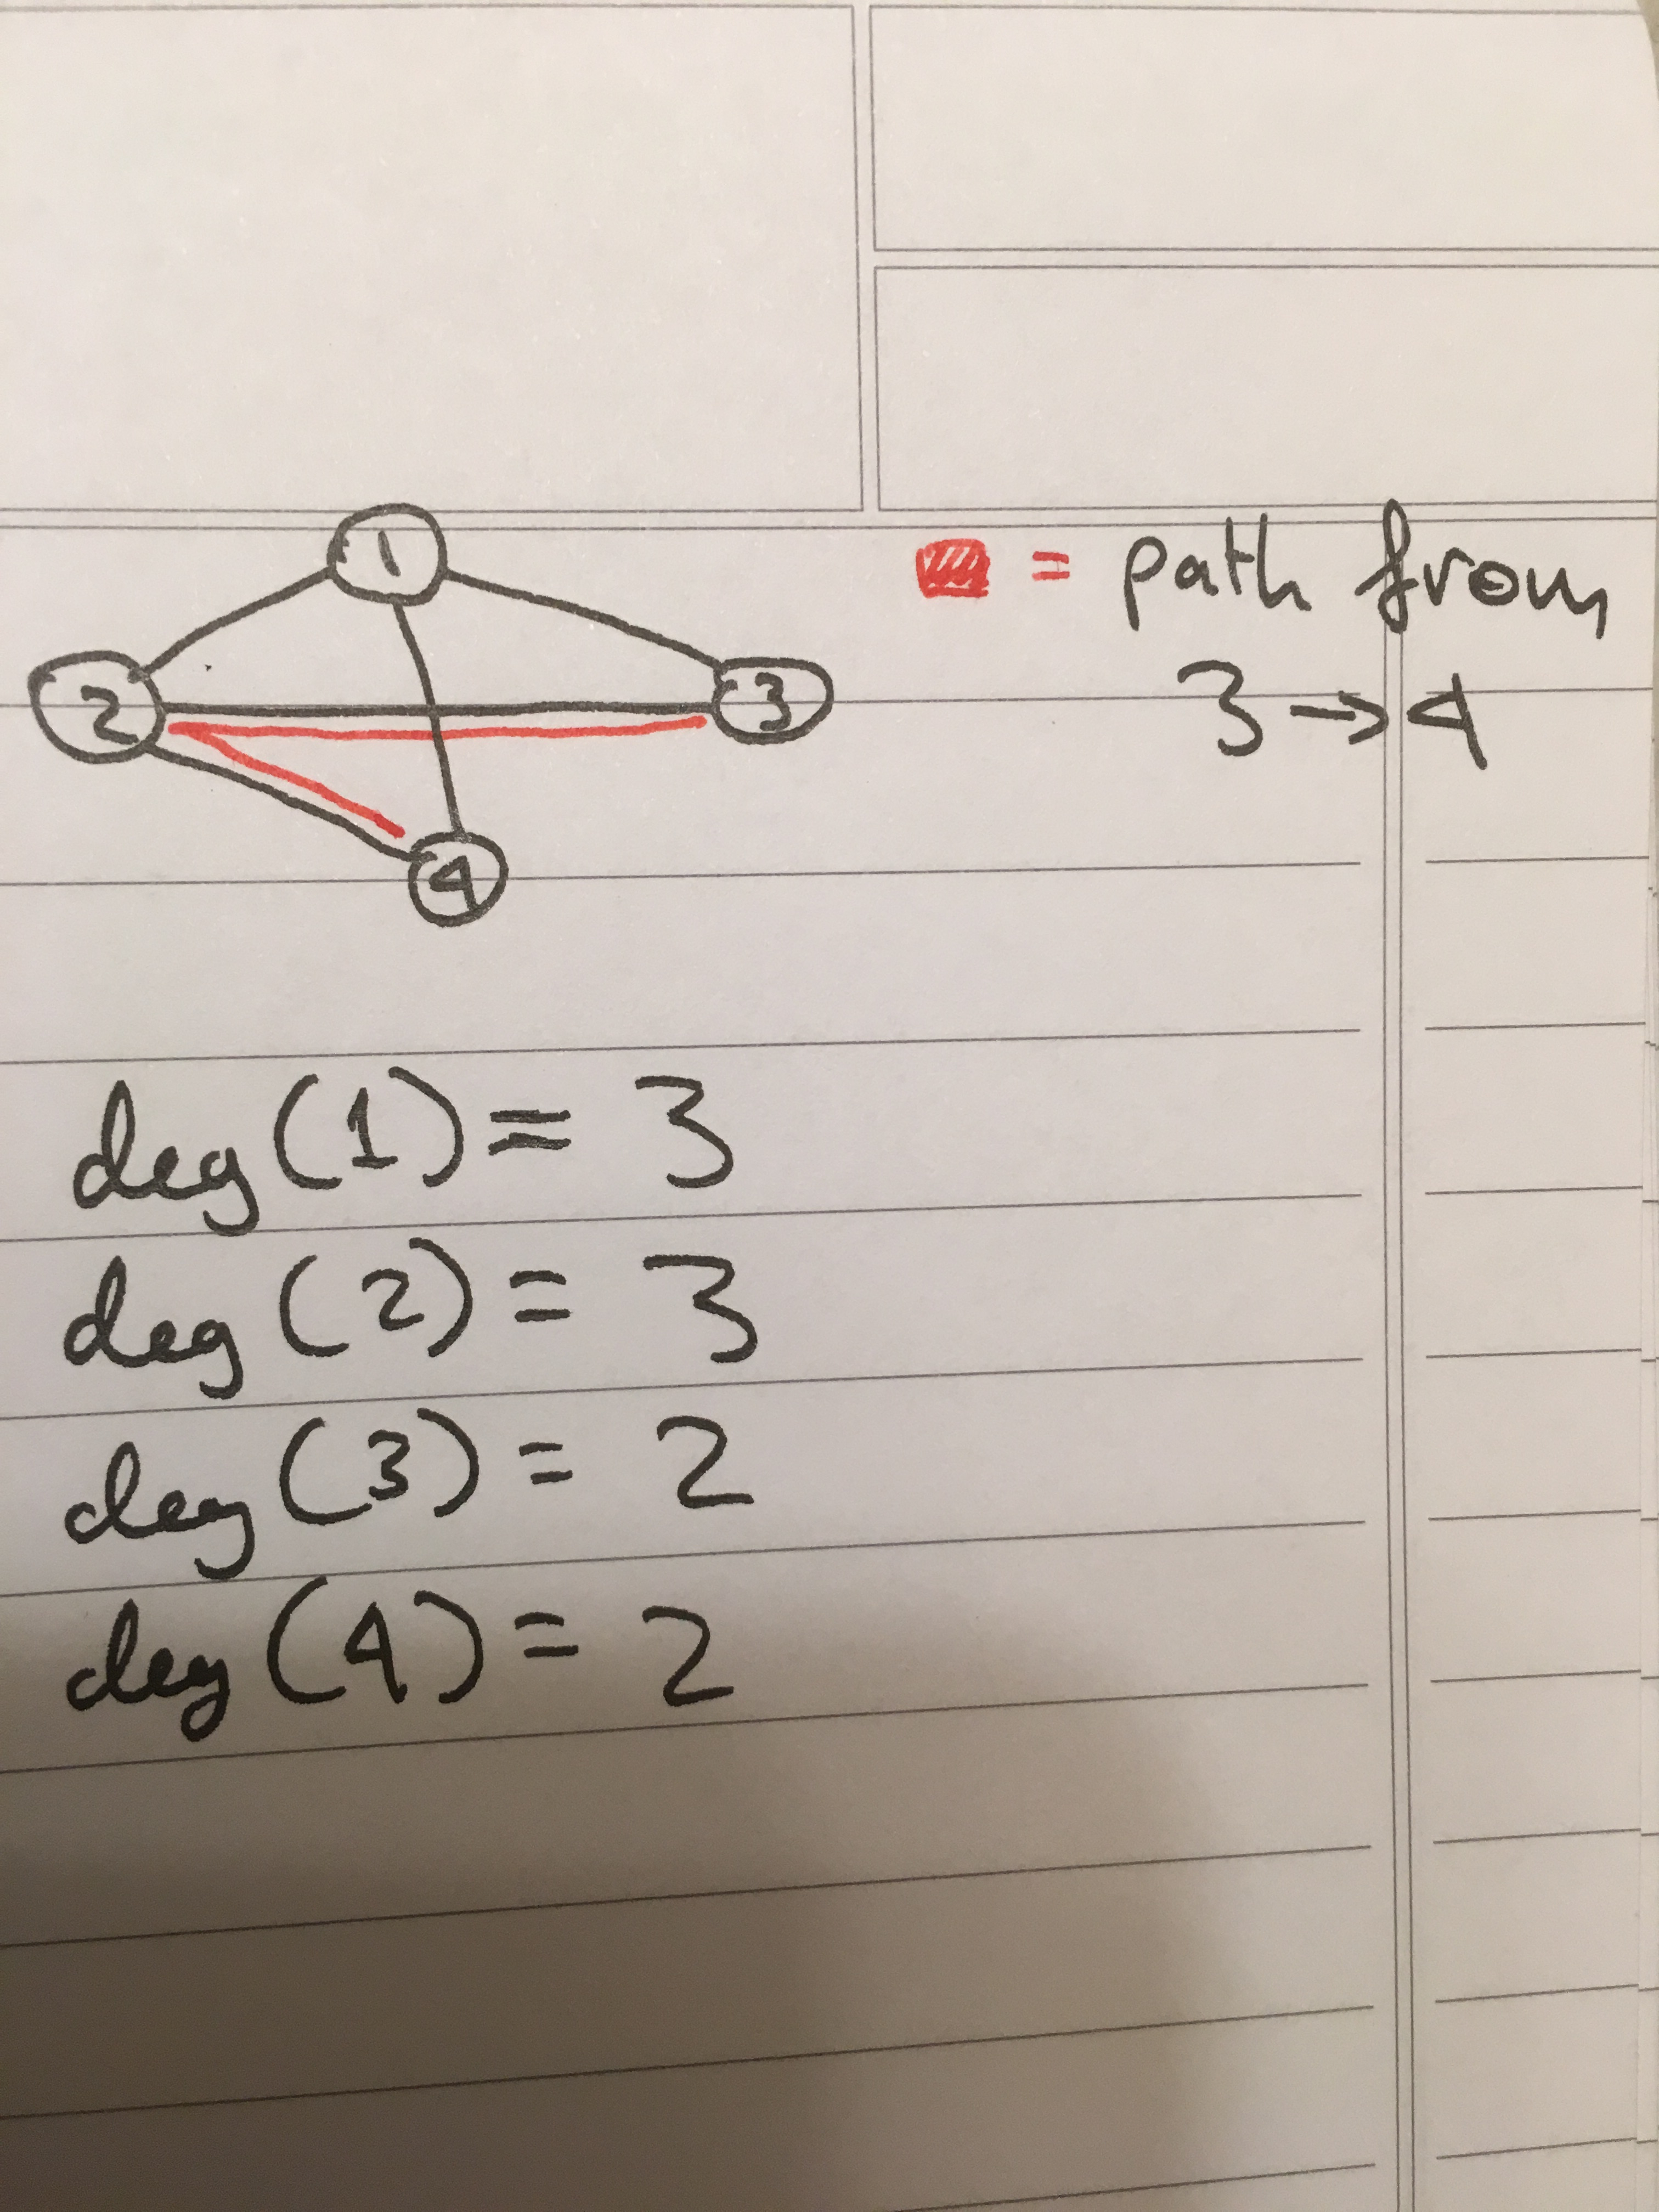
\includegraphics[width=10cm,height=10cm,keepaspectratio]{exer08} \end{center}

\pagebreak
\subsection*{0.9}
Write a formal description of the following graph.
\begin{center} 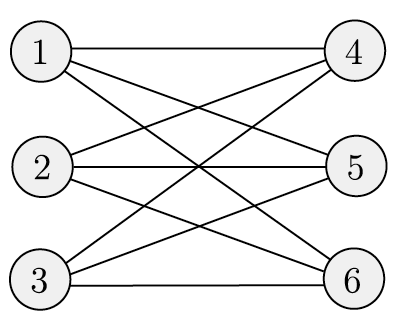
\includegraphics[width=6cm,height=6cm,keepaspectratio]{exer09} \end{center}
\{\{1, 2, 3, 4, 5, 6\}, \{(1, 4), (1, 5), (1, 6), (2, 4), (2, 5), (2, 6), (3, 4), (3, 5), (3, 6)\}\}

\section{Problems page 27 in 3rd ed 0.10, 0.12 and 0.13.}
\subsection*{0.10}
\begin{enumerate}
\item $a = b$
\item $a^2 = ab$
\item $a^2 - a^b = ab - b^2$
\item $\frac{(a + b)(a - b)}{(a - b)} = \frac{b(a - b)}{(a - b)}$
\item $a + b = b$
\end{enumerate}
\begin{claim*} Step 4 is invalid in the case where $a = b = 1$. \end{claim*}
\begin{proof} If $a = b = 1$, that means the term $(a - b) = 0$. This means that (4) is dividing by $0$, an impossible operation. Thus, this is not a proof that $2 = 1$. \end{proof}

\subsection*{0.12}
\begin{claim*} This proof falls apart because it assumes the truth of $k = 2$. \end{claim*}
\begin{proof}
This proof relies heavily on the "middle" set $H_1$, which contains all $k-$horses except the first and the last. However, at just $k = 2$, where the only horses are the first and the last, this "middle" argument falls apart completely. The proof must first establish this base case of $k = 2$ first, before proceeding to larger $k$ values.
\end{proof}

\subsection*{0.13}
Show that every graph with two or more nodes contains two nodes that have equal degrees.\\
We will prove this via Proof by Contradiction.
\begin{proof}
Assume some graph $G = (V, E)$, such that all degrees of nodes in $V$ are distinct. Thus, the set of all possible degrees is $D = \{0, 1, 2, ... , n -1\}$. This means that there is some node $V_i$ with degree $D_i = 0$, and some node $V_j$ with degree $D_j = n-1$. However, $D_i = 0$ implies that there are no edges leaving this node, but $D_j$ implies that node $V_j$ is connected to every node in $G$, other than itself. This is a contradiction of our initial assumption. $\therefore$ there are at least two nodes $\{V_i, V_j\}$ s.t. $D_i = D_j$.
\end{proof}

\section{Prove from the definitions of set union, intersection, complement and equality that:}
\begin{equation}
\overline{(A \cap B)} = (\bar{A} \cup \bar{B})
\end{equation}

\begin{claim*} $\overline{(A \cap B)} \implies (\bar{A} \cup \bar{B})$ \end{claim*}
\begin{proof}
Consider some $x \in \overline{(A \cap B)}$.
\begin{enumerate}[(1)]
\item $x \notin (A \cap B)$
\item $x \in \bar{A} \wedge x \in \bar{B}$
\item $x \notin A \wedge x \notin B$
\item $x \in (\bar{A} \cup \bar{B})$
\end{enumerate}
\end{proof}

\begin{claim*} $(\bar{A} \cup \bar{B}) \implies \overline{(A \cap B)}$ \end{claim*}
\begin{proof}
Consider some $x \in (\overline{A} \cup \overline{B})$.
\begin{enumerate}[(1)]
\item $x \in \overline{A} \lor x \in \overline{B}$
\item $x \notin A \lor x \notin B$
\item $x \in (\overline{A \cap B})$
\end{enumerate}
\end{proof}

Thus, we can see that $\overline{(A \cap B)} = (\bar{A} \cup \bar{B})$.

\section{Show the set of odd numbers is countable.}
The set of odd integers is a subset of the integers (which are countable), it is as most countable.

\section{Prove by induction on $n$.}
\subsection*{Base Case:}
Show that $n = 1$ is true.
\begin{enumerate}
\item $i^2 = \frac{n(n+1)(2n+1)}{6}$
\item $1^2 = \frac{1(1+1)(2(1)+1)}{6}$
\item $1 = \frac{(1)(2)(3)}{6}$
\item $1 = 1$
\end{enumerate}

\subsection*{Inductive Hypothesis:}
\begin{equation}
\text{Assume that} \sum^{k}_{i=1}{i^2} = \frac{k(k+1)(2k+1)}{6} \text{for some} k \in \mathbb{N}
\end{equation}
\subsection*{Inductive Step:}
\begin{claim} If $n = k$ is true, then $n = k + 1$ is also true. \end{claim}
\begin{proof}
For $n = k + 1$, the summation is:
\begin{equation}
\sum^{k + 1}_{i = 1}{i^2}
\end{equation}
Using our inductive hypothesis, we can rewrite this as:
\begin{equation}
\sum^{k}_{i = 1}{i^2} + (k + 1)^2 = \frac{k(k+1)(2k+1)}{6} + (k+1)^2
\end{equation}
\begin{itemize}
\item $\frac{1}{6}(k + 1)k(2k + 1) + (k + 1)(k + 1)$
\item $\frac{1}{6}(k + 1)[k(2k + 1) + 6k + 6]$
\item $\frac{1}{6}(k + 1) [2k^2 + 7k + 6]$
\item $\frac{1}{6}(k + 1) [2k(k + 2) + 3(k + 2)]$
\item $\frac{1}{6}(k + 1)(k + 2)[2k + 3]$
\item $\frac{(k + 1)((k + 1) + 1)(2(k + 1) + 1)}{6}$
\end{itemize}

Which is proof for $n = k + 1$ being true assuming $n = k$. Thus, by proof of induction the statement is true.
\end{proof}
\end{document}
